\documentclass[../main.tex]{subfiles}
\begin{document}
\setchapterstyle{kao}
\setchapterpreamble[u]{\margintoc}
\setchapterimage[6.5cm]{Images/symmqft.jpg}
\chapter[Symmetries in Quantum Field Theory]{Symmetries in Quantum Field Theory\footnotemark[0]}
\labch{symmqft}
\section{The \href{https://en.wikipedia.org/wiki/Eugene_Wigner}{Wigner}-\href{https://en.wikipedia.org/wiki/Hermann_Weyl}{Weyl} Realization}
In Quantum Mechanics, physical states are \textbf{rays} of a \href{https://en.wikipedia.org/wiki/David_Hilbert}{Hilbert} space,\\
$\pazocal{R}=\{e^{i\lambda}\ket{\alpha};\lambda\in\mathbb{R}\}$. A space of rays is called the \textbf{projective Hilbert space}, not a vector space. A symmetry transformation is a change in our point of view that does not change the result of possible experiments: the \textbf{Wigner-Weyl symmetry realization} is a transformation of rays into rays that leaves the transition probabilities constant.
\[
T:\pazocal{R}\to\pazocal{R}' \;\text{such that}\;p(\pazocal{R}_1\to\pazocal{R}_2)=p(\pazocal{R}'_1\to\pazocal{R}'_2)
\]
Instead of working with rays, it is easier to work with the states $\ket{\alpha}$: $T:\ket{\alpha}\to U(T)\ket{\alpha}$. The transition probability must stay the same by definition, so that we have:
\[
|\braket{\alpha_1}{\alpha_2}|=|\braket{\alpha'_1}{\alpha'_2}|=|\braket{U\alpha_1}{U\alpha_2}| 
\]
There is a nice theorem proved by Wigner in the early '30s which tells us that:\marginnote{From \cite{W1}, Section 2.2 and Section 2.7.}
\begin{theorem}[Wigner]
Symmetry transformations can be represented on the Hilbert space by either a \textbf{linear} and \textbf{unitary} operator or an \textbf{anti-linear} and \textbf{anti-unitary} operator.
\end{theorem}
Let's have a look at the two cases:
\begin{itemize}
    \item \underline{Linear and unitary}:
    \begin{enumerate}
        \item $\braket{\alpha}{U\lambda\beta}=\lambda\braket{\alpha}{U\beta}\quad\lambda\in\mathbb{C}$
        \item $\braket{\alpha}{U\beta}=\braket{U^\dagger\alpha}{\beta}$
    \end{enumerate}
    \item \underline{Anti-linear and anti-unitary}:
    \begin{enumerate}
        \item $\braket{\alpha}{U\lambda\beta}=\lambda^*\braket{\alpha}{U\beta}\quad\lambda\in\mathbb{C}$
        \item $\braket{\alpha}{U\beta}=\braket{U^\dagger\alpha}{\beta}^*$
    \end{enumerate}
\end{itemize}
In both cases, we have $UU^\dagger=U^\dagger U=\mathbb{1}$: the conditions for unitarity or anti-unitarity both take the form $U^\dagger=U^{-1}$. Continuity demands that any symmetry that can be made by a continuous change of some parameters must be represented by a linear unitary operator rather than an anti-linear anti-unitary one.\marginnote{Symmetries represented by anti-linear anti-unitary operators are less prominent in physics, they all involve time reversal.}\\
% A representation of a symmetry group on a vector space $V$ is a map between elements of the group and linear operators acting on $V$ which preserves the group multiplication:
% \begin{align*}
%     \text{G}&\to\text{GL}(V)\xleftarrow[]{}\text{space of linear operators on $V$}\\
%     g&\to r(g)\xleftarrow[]{}\text{linear operator}
% \end{align*}
% $r(g)$ is such that $r(T_1\cdot T_2)=r(T_1)\cdot r(T_2)$ and $r(e)=\mathbb{1}$. $g\to U(g)$ is a linear representation on the Hilbert space $\mathcal{H}$. Complications arise from the fact that representations are defined on vectors while here we are working with rays. 
The set of symmetry transformations has certain properties that define it as a \textbf{group}: consider now the action of two symmetry transformations on rays.
\[
\pazocal{R}\xrightarrow[T_1]{}\pazocal{R}'\xrightarrow[T_2]{}\pazocal{R}''
\]
$T_1$ is a transformation that takes $\pazocal{R}$ into $\pazocal{R}'$, $T_2$ takes $\pazocal{R}'$ to $\pazocal{R}''$: the result of performing both transformations is another transformation $T_2T_1$ which takes $\pazocal{R}$ to $\pazocal{R}''$. Moreover, a symmetry transformation $T$ which takes $\pazocal{R}$ to $\pazocal{R}'$ has an inverse $T^{-1}$ such that $TT^{-1}=\mathbb{1}$ and there is an identity transformation $T=1$ that leaves the rays unchanged.\\
The \textbf{unitary operators}\marginnote{Focus just on unitary operators for simplicity.} $U(T)$ corresponding to these symmetry transformations have properties that mirror this group structure but with some complications due to the fact that $U(T)$ acts on vectors in the Hilbert space.
\[
\ket{\alpha}\xrightarrow[T_1]{}U(T_1)\ket{\alpha}\xrightarrow[T_2]{}U(T_2)U(T_1)\ket{\alpha}
\]
$\ket{\alpha}\in\pazocal{R}$, $U(T_1)\ket{\alpha}\in\pazocal{R}'$ and $U(T_2)U(T_1)\ket{\alpha}\in\pazocal{R}''$ but also\\
$U(T_1\cdot T_2)\ket{\alpha}\in\pazocal{R}''$. The last one is not a requirement over the states but over the rays, so the states can differ by a \textbf{phase factor} and this is acceptable. \raisebox{-\mydepth}{{
\includegraphics[height=1.1\baselineskip]{Images/smile.jpg}}}
\[
U(T_2)U(T_1)\ket{\alpha}=e^{i\phi(T_1,T_2)}U(T_1\cdot T_2)\ket{\alpha}
\]
The linearity of the unitary operator\marginnote{Same reasoning apply for the anti-linear operator.} tells us that this phase $\phi$ does not depend on the state $\ket{\alpha}$. To prove that, take two linear independent states, namely $\ket{\alpha}$ and $\ket{\beta}$.
\begin{align*}
e^{i\phi_{\alpha+\beta}(T_1,T_2)}U(T_1\cdot T_2)(\ket{\alpha}+\ket{\beta})&=U(T_2)U(T_1)(\ket{\alpha}+\ket{\beta})\\
&=U(T_2)U(T_1)\ket{\alpha}+U(T_2)U(T_1)\ket{\beta}\\
&=e^{i\phi_a(T_1,T_2)}U(T_1\cdot T_2)\ket{\alpha}+e^{i\phi_\beta(T_1,T_2)}U(T_1\cdot T_2)\ket{\beta}
\end{align*}
Any unitary operator has an inverse which is also unitary, so we multiply both sides on the left by $U^{-1}(T_1\cdot T_2)$:
\[
e^{i\phi_{\alpha+\beta}(T_1,T_2)}(\ket{\alpha}+\ket{\beta})=e^{i\phi_a(T_1,T_2)}\ket{\alpha}+e^{i\phi_\beta(T_1,T_2)}\ket{\beta}
\]
Since $\ket{\alpha}$ and $\ket{\beta}$ are linearly independent, this is only possible if:
\[
e^{i\phi_{\alpha+\beta}}=e^{i\phi_\alpha}=e^{i\phi_\beta}
\]
As promised, the phase is then independent on the state, therefore we can write it as an operator relation:
%for the representation this means that we have \textbf{projective representations}:
\begin{equation}
\labeq{prorep}
U(T_1)U(T_2)=e^{i\phi(T_1,T_2)}U(T_1\cdot T_2)
\end{equation}
For a general phase we have what is called a \textbf{projective representation}, or a representation \textit{up to a phase}. Suppose to have two different classes of phases: we cannot use this rule because the phase in different classes might be different, e.g. when we treat bosons and fermions we cannot take a combination of them because they satisfy different properties (respectively, commutation and anti-commutation rules).

The structure of the Lie group cannot tell us whether the states give a projective representation but it can tell us whether the group has any intrinsically projective representation. There is a kind of group known as \textbf{connected Lie groups} which is of particular importance in physics. These are groups of transformations $T(\theta)$ described by a finite set of real continuous parameters $\theta^a$, with each element of the group connected to the identity by a path which lies in the group. The group multiplication law is in the form:
\[
T(\theta_1)T(\theta_2)=T(f(\theta_1,\theta_2))
\]
Taking $\theta^a=0$ as the coordinates of the identity, we must have:
\[
f^a(\theta,0)=f^a(0,\theta)=\theta^a
\]
As we have said before, the transformations of such groups must be represented by a unitary operator $U(T(\theta))$. For a Lie group, these operators can be represented in a finite neighbourhood of the identity by a power series.
\[
U(T(\theta))=1+i\theta^at_a+\frac{1}{2}\theta^b\theta^ct_{bc}+\dots
\]
where $t_a, t_{bc}=t_{cb}$ and so on are Hermitian operators which do not depend on $\theta$. Suppose now that these operators form an ordinary, i.e. \textit{not} projective, representation of this group of transformations:
\[
U(T(\theta_1))U(T(\theta_2))=U(T(f(\theta_1,\theta_2)))
\]
\marginnote{$f^a(\theta_1,\theta_2)=\theta_1^a+\theta_2^a+f^a_{bc}\theta_1^b\theta_2^c+\dots$}
Expanding this in powers of $\theta_1$ and $\theta_2$ gives us:
\begin{align*}
&\left[1+i\theta_1^at_a+\frac{1}{2}\theta_1^b\theta_1^ct_{bc}+\dots\right]\left[1+i\theta_2^at_a+\frac{1}{2}\theta_2^b\theta_2^ct_{bc}+\dots\right]\\
=&1+i(\theta_1^a+\theta_2^a+f^a_{bc}\theta_1^b\theta_2^c+\dots)t_a+\frac{1}{2}(\theta_1^b+\theta_2^b+\dots)(\theta_1^c+\theta_2^c+\dots)t_{bc}+\dots
\end{align*}
From this, by comparing equal order terms we get a non-trivial condition:
\[
t_{bc}=-t_bt_c-if^a_{bc}t_a
\]
This shows that if we are given the structure of a group, we can calculate the second-order terms in $U(T(\theta))$ from the generators $t_a$ appearing in the first-order terms. However, there is a consistency condition: $t_{bc}$ must be symmetric in $b$ and $c$\marginnote{It is the second derivative of $U(T(\theta))$ with respect to $\theta_1$ and $\theta_2$.}. This requires that:
\begin{align*}
[t_b,t_c]&=t_bt_c-t_ct_b=\cancel{-t_{bc}}-if^a_{bc}t_a+\cancel{t_{cb}}+if^a_{cb}t_a\\
&=i(f_{cb}^a-f_{bc}^a)t_a=iC_{bc}^at_a
\end{align*}
$C^a_{bc}$ are a set of real constants known as \textbf{structure constants}. Such set of commutation relations is called a \textbf{Lie algebra}. We are going to see that this commutation relation is the single condition needed to ensure that this process continues: the power series of $U(T(\theta))$ may be calculated from an infinite sequence of relations provided we know the first-order terms $t_a$.\\
Suppose that $f(\theta_1,\theta_2)$ is simply additive. The coefficient $f^a_{bc}$ vanishes and so does the structure constant: this implies that the generators commute, $[t_b,t_c]=0$. Here it is easier to calculate $U(T(\theta))$ for all $\theta^a$:
\[
U(T(\theta))=\left[U\left(T\left(\frac{\theta}{N}\right)\right)\right]^N\xrightarrow[N\to\infty]{}\exp{it_a\theta^a}
\]
How can we understand if a group of symmetry has a projective representation? The basic requirement that any phase in \refeq{prorep} would have to satisfy is associativity:
\[
U(T_3)(U(T_2)U(T_1))=(U(T_3)U(T_2))U(T_1)
\]
which imposes on $\phi$ the following condition:
\begin{equation}
\labeq{phicond}
\phi(T_2,T_1)+\phi(T_3,T_2T_1)=\phi(T_3,T_2)+\phi(T_3T_2,T_1)
\end{equation}
Any phase of the form:
\begin{equation}
\labeq{phiform}
\phi(T_1,T_2)=\alpha(T_1T_2)-\alpha(T_1)-\alpha(T_2)
\end{equation}
would satisfy this condition, but a projective representation with such a phase can be replaced with an ordinary representation by simply defining \\
$\Tilde{U}(T):=U(T)\exp{i\alpha(T)}$. Any set of functions $\phi(T_1,T_2)$ which satisfies \refeq{phicond} and differs by a function $\Delta\phi(T_1,T_2)$ of the form \refeq{phiform} is called a \textbf{two-cocycle}. We are interested in whether a symmetry group allows any non-trivial two-cocycle\marginnote{A trivial cocycle is one containing $\phi=0$.}, i.e. whether it may have a representation on the Hilbert space that is intrinsically projective, in the sense that the phase $\phi(T_1,T_2)$ cannot be eliminated in this way.\\
When either $T_1$ or $T_2$ is the identity the phase must vanish, when both are near the identity the phase must be small:
\[
\phi(T(\theta_1),T(\theta_2))=f_{ab}\theta_1^a\theta_2^b+\dots
\]
Inserting this expansion in the power series of \refeq{prorep}, we get:
\[
[t_b,t_c]=iC^a_{bc}t_a+iC_{bc}\mathbb{1} \quad C_{bc}:=-f_{bc}+f_{cb}
\]
$C_{bc}$ is the \textbf{asymmetry coefficient}, the terms proportional to this coefficient are called \textbf{central charges}. $C_{bc}$ and $C_{bc}^a$ are subject from an important constraint coming from Jacobi identity: we take the sum $[[t_b,t_c],t_d]+[[t_c,t_d],t_b]+[[t_d,t_b],t_c]$. This gives us:
\[
C^a_{bc}C^e_{ad}+C^a_{cd}C^e_{ab}+C^a_{db}C^e_{ac}=0 \quad C^a_{bc}C_{ad}+C^a_{cd}C_{ab}+C^a_{db}C_{ac}=0
\]
The equation on the right has one class of non-zero solutions given by $C_{ab}=C^e_{ab}\phi_e$, with $\phi_e$ a set of real constants. For these solutions, we can eliminate the central charges by redefining the generators\\
$t_a\to\Tilde{t}_a=t_a+\phi_a$. These new generators now satisfy the following commutation rule without central charges:
\[
[\Tilde{t}_b,\Tilde{t}_c]=iC^a_{bc}\Tilde{t}_a
\]
We are now ready to state the theorem that governs the occurrence of intrinsically projective representations. The phase $\phi$ of any representation $U(T)$ of a given group can be chosen to be $\phi=0$ if two conditions are satisfied:
\begin{enumerate}
    \item The generators of the group in this representation can be defined in such a way to eliminate all central charges from the Lie algebra.
    \item The group is \textbf{simply connected}\marginnote[-0.5cm]{An equivalent statement is that any loop which starts and end at the same element of the group can be continuously shrunk to a point.}, i.e. any two elements of the group can be connected by a path lying within the group and any two such paths may be continuously transformed one into another.\\
    e.g. \marginnote{For every not simply connected group there exists a \textbf{universal covering} which is a simply connected group with the same algebra. In these examples, the universal covering of SO(3) is SU(3), the universal covering of SO(3,1) is SL$(2,\mathbb{C})$.}SO(3)$\sim S^3/\mathbb{Z}_2$ is a 3D sphere with equal antipodal points, it is not simply connected. The two antipodal points are the same point physically speaking, they come from the same rotation. The phase $\phi=0$ for bosonic states, while $\phi=\pm\pi$ on fermionic states. The \href{https://en.wikipedia.org/wiki/Hendrik_Lorentz}{Lorentz} group given by SO(3,1)$\sim\mathbb{R}\times S^3/\mathbb{Z}_2$ is not simply connected either.
\end{enumerate}
This shows that there are two ways in which intrinsically projective representations may arise: algebraically, because the group is represented projectively even near the identity, or topologically, because the group is not simply connected, hence a path from 1 to $T_1$ and from $T_1$ to $T_2$ may not be continuously deformable into another path from 1 to $T_1T_2$.

\subsection{Implications of Wigner-Weyl Symmetry}
% Suppose now that such a representation $U(g)$ exists: the action of the symmetry transformation on the algebra of observables is \textbf{linear}. We have a state $\ket{\alpha}$: we can perform a rotation of the state without touching the reference system.
% \[
% \ket{\alpha}\to\ket{\alpha_g}=\bra{\alpha_g}A\ket{\alpha_g}
% \]
% Another possibility is to rotate the reference system without touching the state instead, $\bra{\alpha}A_{g^{-1}}\ket{\alpha}$. These two possibilities must give the same result:
% \[
% \ket{\alpha_g}=U(g)\ket{\alpha}\Rightarrow\bra{\alpha_g}A\ket{\alpha_g}=\bra{\alpha}U^\dagger(g)AU(g)\ket{\alpha}
% \]
% Hence, we can identify the transformation:
% \[
% A\xrightarrow[g]{}A_g=U(g)AU^\dagger(g)\quad U(g^{-1})=U^\dagger(g)
% \]
% Suppose to have not one, but a series of observables $A_i$ and transform them under $g$:
% \[
% A_i\xrightarrow[g]{}A_{ig}=U(g)A_iU^\dagger(g)=\underset{\mathclap{\tikz \node {$\uparrow$} node [below=1ex] {\footnotesize  representation of the algebra of observables};}}{R_{ij}}A_j
% \]
% Consider an infinitesimal transformation, we can express $R_{ij}$ as the identity+the generators of the algebra:
% \[
% R_{ij}(\alpha)=\delta_{ij}+it_{ij}^a\alpha^a+\pazocal{O}(\alpha^2)
% \]
% The same is true for the fields, $\phi_i(x)=U(g)\phi_i(x)U^\dagger(g)=R°{ij}\phi_j(x)$.\\
A consequence of the Wigner-Weyl symmetry realization is that the charge, if it is well defined, is the \textbf{generator} of the symmetry, which means that it is possible to write $U(g(\alpha))=\exp{iQ^a\alpha^a}$. In the classical theory, we know that:
\[
Q^a=\int d^3xJ^{0,a}(\Vec{x},t) \quad \{Q^a,\phi_i(\Vec{x},t)\}=\frac{\partial\phi_i(\Vec{x},t)}{\partial x} \quad \phi_i(x)\to\phi_i(x)+\alpha\frac{\partial\phi_i}{\partial x}
\]
We want to do the same in Quantum Field Theory (QFT). Assume that there are some generators $G^a$, and take $\phi\to\phi'=U\phi U^\dagger$. Consider now the infinitesimal form of this transformation:
\[
(\mathbb{1}+i\alpha^aG^a)\phi_i(x)(\mathbb{1}-i\alpha^aG^a)=\phi_i(x)+it_{ij}^a\alpha^a\phi_j(x)
\]
where we used the fact that $[G^a,\phi_i(x)]=t_{ij}^a\phi_j(x)$. In the classical theory, the charge is always well defined since the current density makes the integral convergent. However, this is generally not true in QFT, since the Lagrangian involves operators of fields in the same space-time point and these quantities are not always well defined. For example, to regularize the integral we usually put a finite lower limit and then we send it to infinity:
\[
Q^a=\lim_{V\to\infty}\int_V d^3xJ^{0,a}(\Vec{x},t)=\lim_{V\to\infty}Q_V^a(t)
\]
where the current is defined as:
\[
J^{0,a}(x)=\frac{\delta\pazocal{L}}{\delta\Dot{\phi}_i(x)}it_{ij}^a\phi_j(x)=\pi_i(x)it_{ij}^a\phi_j(x)
\]
One way to see that $Q^a$ is a generator is to use the properties of the generators, i.e. the structure of the algebra. We make use of equal time commutation relation, $[\pi_i(\Vec{x},t),\phi_j(\Vec{y},t)]=i\delta_{ij}\delta^3(\Vec{x}-\Vec{y})$ and commutator properties for the following computation.\marginnote{This is my best attempt in making the calculation works.}
\begin{align*}
[Q^a,Q^b]&=\int d^3xd^3y[J^{0,a}(\Vec{x},t),J^{0,b}(\Vec{y},t)]\\
&=\int d^3xd^3y[\pi_i(\Vec{x},t)it_{ij}^a\phi_j(\Vec{x},t),\pi_k(\Vec{y},t)it_{kl}^b\phi_l(\Vec{y},t)]\\
&=-\int d^3xd^3y\left\{\pi_i(\Vec{x},t)t_{ij}^a[\phi_j(\Vec{x},t),\pi_k(\Vec{y},t)]t_{kl}^b\phi_l(\Vec{y},t)+\pi_k(\Vec{y},t)t_{kl}^b[\pi_i(\Vec{x},t),\phi_l(\Vec{y},t)]t_{ij}^a\phi_j(\Vec{x},t)\right\}\\
&=-\int d^3xd^3y\left[-\pi_i(\Vec{x},t)t_{ij}^ai\delta_{jk}\delta^3(\Vec{x}-\Vec{y})t_{kl}^b\phi_l(\Vec{y},t)+\pi_k(\Vec{y},t)t_{kl}^bi\delta_{il}\delta^3(\Vec{x}-\Vec{y})t_{ij}^a\phi_j(\Vec{x},t)\right]\\
&=-i\int d^3x\left[-\pi_i(x)t_{ij}^at_{jl}^b\phi_l(x)+\pi_k(x)t_{kl}^bt_{lj}^a\phi_j(x)\right]\\
&=+i\int d^3x\left\{\pi_i(x)[t^a,t^b]_{il}\phi_j(x)\right\}\\
&=+if^{abc}\int d^3x\pi_i(x)it_{il}^c\phi_l(x)=+if^{abc}Q^c \quad \checkmark
\end{align*}
This is the \textbf{charge algebra}. If we work with currents instead, we obtain something similar:
\[
[J^{0,a}(\Vec{x},t),J^{0,b}(\Vec{y},t)]=if^{abc}J^{0,c}(\Vec{x},t)\delta^3(\Vec{x}-\Vec{y})
\]
% At equal times, we have local properties, but in principle we could have higher order terms involving derivatives and delta functions. There are some cases in which these terms must exist, let's look at a general case:
% \[
% [J^{0,a}(\Vec{x},t),J^{i,b}(\Vec{y},t)]=if^{abc}J^{i,c}(\Vec{x},t)\delta^3(\Vec{x}-\Vec{y})+S^{ab}(\Vec{x})\frac{\partial}{\partial x^i}\delta^3(\Vec{x}-\Vec{y})
% \]
% The extra-term is called the \href{https://en.wikipedia.org/wiki/Julian_Schwinger}{Schwinger} term. Only in particular cases we do not have higher order terms, generally for each operator with local properties at equal time we have higher order terms.

What are the consequences of the Wigner-Weyl symmetry? We know that the charges are the generator, so now we bring our attention to the behaviour of the vacuum under symmetry. 
\begin{theorem}(Fabri-Picasso)
\labthm{FP}
If the vacuum is \textbf{not invariant} under symmetry transformation, then the charge $Q^a$ is \textbf{not well defined}.
\[
Q^a\ket{0}\neq0\Rightarrow Q^a=\lim_{V\to\infty}\int_Vd^3xJ^{0,a}(\Vec{x},t)=\lim_{V\to\infty}Q_V^a(t)\to\infty
\]
\end{theorem}
\begin{proof}
Consider a single charge $Q$ acting on the vacuum $\ket{0}$ and compute its norm.
\[
\norm{Q\ket{0}}^2=\bra{0}QQ\ket{0}=\int d^3x\bra{0}J^0(\Vec{x},t)Q\ket{0}
\]
We can use the fact that $J^0(x)=e^{-ipx}J^0(0)e^{+ipx}$:
\[
\bra{0}J^0(\Vec{x},t)Q\ket{0}=\underbrace{\bra{0}e^{-ipx}}_{\bra{0}e^{-iE_0t}}J^0(0)\underbrace{e^{+ipx}Qe^{-ipx}}_{Q}\underbrace{e^{+ipx}\ket{0}}_{e^{+iE_0t}\ket{0}}=\bra{0}J^0(0)Q\ket{0}
\]
This quantity is independent on $x$, therefore when taking the integral there are some problems:
\[
\lim_{V\to\infty}\int_Vd^3x\bra{0}J^0(0)Q\ket{0}\to\infty
\]
\end{proof}
On the other hand, if the vacuum is invariant, i.e. $Q^a\ket{0}=0$, then the physical states are classified in degenerate multiplets of the symmetry, which means that they belong to groups of states with the same energy. Suppose to have a state $\ket{\alpha_i}=A_i\ket{0}$, with $A_i$ local operator which excites the vacuum. We want to show that also $A_i$ transforms as an element of the multiplet.
\[
A_i\to U(g)A_iU^\dagger(g)=R_{ij}A_j
\]
Define now the state $\ket{\beta_i}$ as the action of $R_{ij}A_j$ on the vacuum $\ket{0}$.
\[
\ket{\beta_i}=R_{ij}A_j\ket{0}=U(g)A_iU^\dagger(g)\ket{0}=U(g)A_i\ket{0}=U(g)\ket{\alpha_i}
\]
It is possible to conclude that these states are \textbf{degenerate}:
\[
E_{\beta_i}=\bra{\beta_i}H\ket{\beta_i}=\bra{\alpha_i}U^\dagger(g)HU(g)\ket{\alpha_i}\underset{\mathclap{\tikz \node {$\uparrow$} node [below=1ex] {\footnotesize \underline{if $[H,U(g)]=0$} };}}{=}\bra{\alpha_i}H\ket{\alpha_i}=E_{\alpha_i}
\]
The only thing left to prove is that if the vacuum is invariant, then $[H,U(g)]=0$. This is known as the \href{https://en.wikipedia.org/wiki/Sidney_Coleman}{Coleman} theorem.
\begin{theorem}[Coleman]
\labthm{Coleman}
If the vacuum is invariant, then the current is conserved.
\[
\partial_\mu J^\mu=0 \quad \text{and}\;[H,Q]=0
\]
For a well defined charge $Q$.
\end{theorem}
\begin{proof}
The vacuum is invariant, which means that:
\[
Q\ket{0}=\int d^3xJ^0(\Vec{x},t)\ket{0}=0
\]
We multiply the integrand on the left by a generic state $n$ with zero three momentum:
\[
\bra{n,\vec{p}_n=0}J^0(\Vec{x},t)\ket{0}=\underbrace{\bra{n,p_n}e^{-ipx}}_{\bra{n,\Vec{p}_n=0}}J^0(\Vec{0},t)\underbrace{e^{+ipx}\ket{0}}_{=\ket{0}}=0
\]
Consider now the derivative with respect to time of $J^0(x)$,\\
$\bra{n,\vec{p}_n=0}\partial_0J^0(x)\ket{0}=0$. This can be written as the total derivative of the current, since the spatial derivative is equal to zero.
\[
\bra{n,\vec{p}_n=0}\Vec{\nabla}\cdot\Vec{J}(\Vec{x})\ket{0}=\bra{n,\vec{p}_n=0}\Vec{\nabla}\cdot(e^{-ipx}\Vec{J}(\Vec{0})e^{+ipx})\ket{0}=\bra{n,\vec{p}_n=0}(-i\Vec{p}\Vec{j}(\Vec{x})+\Vec{J}(\Vec{x})i\Vec{p}\ket{0}=0
\]
We proved that $\bra{n,\vec{p}_n=0}\partial_\mu J^\mu\ket{0}=0$. Moreover, the operator is \textbf{Lorentz invariant} so we can perform a boost to end up in a reference system where the momentum $\vec{p}_n$ is different from zero. We have a state whose projection on all possible states is zero, this imply that:
\[
\partial_\mu J^\mu\ket{0}=0
\]
There is a nice theorem\marginnote{Contino didn't say which was this \textit{nice theorem}. I personally doubt it exists, adding material to the thesis that this course was a scam.} which tells us that if $O(x)\ket{0}=0$ for $O(x)$ local, then $O(x)=0$. Using this result, we have that $\partial_\mu J^\mu=0$. From this fact, we can proceed as in the classical way to prove that the charge is conserved, hence $\frac{dQ}{dt}=[H,Q]=0$.
\end{proof}
% In Quantum Electrodynamics (QED), electric charges form a multiplet of degenerate states, coming from a Wigner-Weyl symmetry. Every state has a specific electric charge (this is why $e^-$ has charge -1 and $\gamma$ has charge zero). Now we want to see this from a different point of view, using \href{https://en.wikipedia.org/wiki/George_Green_(mathematician)}{Green}'s functions. Consider the following object:
% \[
% \bra{0}T[J^{\mu,a}(x)\phi_{i_1}(x_1)\dots\phi_{i_n}(x_n)]\ket{0}
% \]
% We derive it with respect to $\partial_\mu^x$:
% \[
% \partial_\mu^x\bra{0}T[J^{\mu,a}(x)\phi_{i_1}(x_1)\dots\phi_{i_n}(x_n)]\ket{0}=\sum_{i=1}^n\bra{0}T[\phi_{i_1}(x_1)\dots\underbrace{t^a\phi(x)}_{\text{i-th term}}\dots\phi_{i_n}(x_n )]\ket{0}\delta^3(\Vec{x}-\Vec{x}_i)
% \]
% The delta comes from the derivative of the theta function inside the T-product.
\section{Approximate Symmetries and Spurion Analysis}
Spurion analysis consists basically in a fictitious auxiliary field which can be used to parametrize spontaneous symmetry breaking and determine all the invariant operators under that symmetry. The procedure begins with finding a parameter that measures the amount of symmetry breaking. This parameter is then promoted to a field, i.e. to a function of the space-time coordinates. With this new fictitious field, operators that are invariant under the symmetry may be found by the usual group-theoretical considerations. The list of operators found in this way is complete as long as all sources of the breaking are included. The operators in the actual theory are ultimately found by setting the spurious field equal to the constant value of the parameter.\\
To make things more clear, consider the case of QED:
\[
\pazocal{L}=-\frac{1}{4}F_{\mu\nu}F^{\mu\nu}+\Bar{\Psi}(i\gamma^\mu D_\mu-m)\Psi
\]
with $D_\mu=\partial_\mu-ieA_\mu$. This Lagrangian has a global U(1) symmetry and an axial U$(1)_A$ symmetry, regarding only the kinetic term:
\[
\text{U}(1):
\left\{
\begin{aligned}
&\Psi(x)\to e^{i\alpha}\Psi(x)\\
&A_\mu\to A_\mu
\end{aligned}
\right.
\quad 
\text{U}(1)_A:
\left\{
\begin{aligned}
&\Psi(x)\to e^{i\alpha\gamma_5}\Psi(x)\\
&A_\mu\to A_\mu
\end{aligned}
\right.
\]
The axial symmetry does not involve the mass term, otherwise the symmetry would be broken. To see that, let's consider a left- and a right-handed fermion defined as follows:
\[
\left\{
\begin{aligned}
&\Psi_L(x)=\frac{1-\gamma_5}{2}\Psi(x)=P_L\Psi(x)\to e^{-i\alpha}\Psi_L(x)\\
&\Psi_R(x)=\frac{1+\gamma_5}{2}\Psi(x)=P_R\Psi(x)\to e^{+i\alpha}\Psi_R(x)
\end{aligned}
\right.
\]
In the transformations we have different phases but the fields are not mixed. We now look at the mass term:
\[
m\Bar{\Psi}\Psi=m(\Bar{\Psi}_L\Psi_R+\Bar{\Psi}_R\Psi_L)\to m(e^{2i\alpha}\Bar{\Psi}_L\Psi_R+e^{-2i\alpha}\Bar{\Psi}_R\Psi_L)
\]
The mass term breaks this symmetry. To overcome the problem, consider the mass as an object which transforms:
\[
m\Bar{\Psi}\Psi\to m\Bar{\Psi}_L\Psi_R+m^*\Bar{\Psi}_R\Psi_L\marginnote{This is a better and more general definition of the mass term.}
\]
The spurion transformation rule tells us that $m\to e^{-2i\alpha}m$, in this way the mass term is invariant and therefore the Lagrangian is invariant under the axial symmetry.\\
% We now want to understand how this new term behaves with this new definition.
% \[
% m\to m+\delta m \quad \text{U}(1)_A:\delta m\to e^{-2i\alpha}\delta m
% \]
% $\delta m$ must be proportional to $m$: we are \textbf{renormalizing} the mass.\marginnote{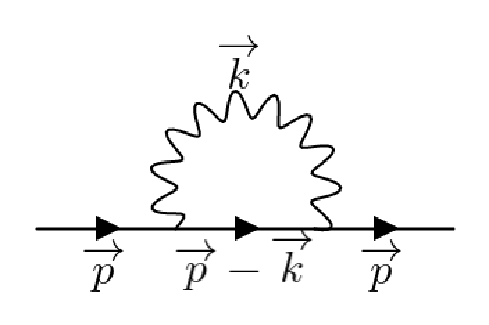
\includegraphics{Images/eselfenergy.pdf}} Naively computing the fermion propagator at first order, we expect a linear divergence for the mass, but the spurion analysis tells us that this divergence is not allowed: we have some problems with our transformations. What we can do is to send the external momentum $p$ to zero and expand around it. Doing this, we expect a logarithmically divergent term which is allowed.\\
We want to go back to the system in which the mass is real, because in order to remove the symmetry breaking we had to introduce a basis in which the mass is complex.
\[
m\Bar{\Psi}_L\Psi_R\to me^{2i\alpha}\Bar{\Psi}_L\Psi_R \quad \alpha=\pi/2: m\to-m
\]
Axial parity allows us to change the sign of the mass without symmetry breaking, but there are theories where this transformation is not allowed. Problems may arise when we have gauge invariance, where this change of sign could create additional effects, anomalies.\\
When we consider global symmetries for a theory of $N$ free fermions, we immediately encounter a complication since there are different types of fermions.
\[
\Psi=\left(\begin{array}{c}
     \xi \\
     \eta
\end{array}\right)
\begin{array}{c}
     \xleftarrow[]{}\text{left-handed field}\\
     \xleftarrow[]{}\text{right-handed field}
\end{array}
\]
Acting with the projection operators let us easily select either the left- or the right-handed field.\marginnote{For the $\gamma$ matrices, we are working in the \href{https://en.wikipedia.org/wiki/Gamma_matrices#Weyl_(chiral)_basis}{Weyl basis}.}
\[
\gamma_5=\mqty(\dmat{-\mathbb{1},\mathbb{1}})
\quad
\Psi_L=\frac{1-\gamma_5}{2}\Psi=
\left(\begin{array}{c}
    \xi \\
     0
\end{array}\right)
\quad
\Psi_R=\frac{1+\gamma_5}{2}\Psi=
\left(\begin{array}{c}
     0 \\
     \eta
\end{array}\right)
\]
\subsection{Representations of the Lorentz Group}
\labsec{replor}\marginnote{From \cite{schwartz}, Section 10.1-10.2.}
The Lorentz group SO(3,1) is \textbf{not compact}: for non-compact groups, finite-dimensional representations are not unitary and unitary representation are infinite-dimensional. We want to understand what are the more convenient representations for $\Psi$. Our goal is to find all the finite-dimensional representations of the Lorentz group, i.e. matrices which represent the action of the group generators on the algebra. Recall that the Lorentz group is the set of boosts and rotations that preserve the Minkowski metric, $\Lambda^T g\Lambda=g$. The $\Lambda$ matrices in this equation are in the 4-vector representation under which we have:
\[
X_\mu\to\Lambda_{\mu\nu}X_\nu
\]
The matrices representing boosts and rotations give an embedding of elements of the Lorentz group into a set of matrices, which means that they describe one particular representation of the Lorentz group (the 4-vector representation). The Lorentz group is a mathematical object independent of any particular representation. To extract the group away from its representations, it is possible to look at infinitesimal transformations which in the 4-vector representation can be written as:
\[
\left\{
\begin{aligned}
&\delta X_0=\beta_iX_i\\
&\delta X_i=\beta_iX_0-\epsilon_{ijk}\theta_jX_k
\end{aligned}
\right.
\]
where we have six infinitesimal angles $\theta_i$ and $\beta_i$. Alternatively, the infinitesimal transformations can be written as:
\[
\delta X_\mu=i\sum_{i=1}^3[\theta_i(J_i)_{\mu\nu}+\beta_i(K_i)_{\mu\nu}]X_\nu
\]
% We know that SO(3,1) has an universal covering which is SL$(2,\mathbb{C})$ and we start by looking at its algebra.
% \[
% \forall x^\mu: X=x^\mu\sigma_\mu\left(\begin{array}{cc}
%     x^0-x^3 & -x^1+ix^2 \\
%     -x^1-ix^2 & x^0+x^3
% \end{array}\right)
% \]
% where $\sigma_\mu=(\mathbb{1},-\Vec{\sigma})$ and $\det X=\norm{x}^2$. In the Lorentz group, $X$ transforms as:
% \[
% X\to X'=\Lambda^\mu_\nu x^\nu\sigma_\mu \quad \det X=\det X'
% \]
% We can also find transformations in SL$(2,\mathbb{C})$ which leaves the determinant invariant:
% \[
% X\to X'=AXA^\dagger \quad A\in\text{SL}(2,\mathbb{C}) \; \det X'=\det X|\det A|^2=\det X
% \]
% We can show that there is a map between elements of SO(3,1), i.e. $\Lambda$, and elements of SL$(2,\mathbb{C})$, i.e. $A$.
% \[
% \Lambda^\mu_\nu x^\nu\sigma_\mu\to Ax^\mu\sigma_\mu A^\dagger
% \]
% In SL$(2,\mathbb{C})$, there are two elements which correspond to $\Lambda$, which are $A$ and $-A$. We therefore have the double of the elements of SO(3,1), so the correct relations between the two groups is SO(3,1)=SL$(2,\mathbb{C})/\mathbb{Z}_2$.\\
where we introduced the \textbf{generators} of the group, corresponding to rotations $J_i$ and boost $K_i$:
\[
\begin{aligned}
&J_1=i\left(\begin{array}{cccc}
     0 & & & \\
     & 0 & & \\
     & & 0 & -1 \\
     & & +1 & 0
\end{array}\right)
&&J_2=i\left(\begin{array}{cccc}
     0 & & & \\
     & 0 & & +1\\
     & & 0 &  \\
     & -1 &  & 0
\end{array}\right)
&&&J_3=i\left(\begin{array}{cccc}
     0 & & & \\
     & 0 & -1 & \\
     & +1 & 0 &  \\
     & &  & 0
\end{array}\right)\\
&K_1=i\left(\begin{array}{cccc}
     0 & -1 & & \\
     -1 & 0 & & \\
     & & 0 &  \\
     & & & 0
\end{array}\right)
&&K_2=i\left(\begin{array}{cccc}
     0 & & -1 & \\
     & 0 & & \\
     -1 & & 0 &  \\
     &  &  & 0
\end{array}\right)
&&&K_3=i\left(\begin{array}{cccc}
     0 & & & -1 \\
     & 0 & & \\
     & & 0 &  \\
     -1 & &  & 0
\end{array}\right)
\end{aligned}
\]
They generate the group in the sense that any element of the group can be written uniquely as:
\[
\Lambda=\exp{i\theta_iJ_i+i\beta_iK_i}
\]
In any finite-dimensional representation the group elements can be written as en exponential of matrices.
By using the expression for the generators provided above, it is possible to calculate the commutation relations. We find:
\[
\left\{
\begin{aligned}
&[J_i,J_j]=i\epsilon_{ijk}J_k\\
&[J_i,K_j]=i\epsilon_{ijk}K_k\\
&[K_i,K_j]=i\epsilon_{ijk}J_k
\end{aligned}
\right.
\]
These commutation relations describe the \textbf{Lorentz algebra} $\mathfrak{so}(3,1)$.\\
The irreducible representations of the Lorentz group can be constructed from irreducible representations of SU(2). The algebraic properties stated above are representations independent, so we can take for example $J_i^\pm:=(J_i\pm iK_i)/2$, which satisfy:
\begin{equation}
\labeq{commrules}
\left\{
\begin{aligned}
&[J_i^+,J_j^+]=i\epsilon_{ijk}J^+_k\\
&[J_i^-,J_j^-]=i\epsilon_{ijk}J_k^-\\
&[J_i^+,J_j^-]=0
\end{aligned}
\right.
\end{equation}
These relations show that the Lie algebra for the Lorentz group has two commuting subalgebras. The algebra generated by $J_i^+$ (or $J_i^-$) is the 3D rotation algebra which has multiple names,\\
$\mathfrak{so}(3)=\mathfrak{sl}(2,\mathbb{R})=\mathfrak{so}(2,1)=\mathfrak{su}(2)$. Therefore, we have shown that:
\[
\mathfrak{so}(3,1)\sim\mathfrak{sl}(2,\mathbb{C})\sim\mathfrak{su}(2)\oplus\mathfrak{su}(2)
\]
This decomposition makes studying the irreducible representations very easy: we know from quantum mechanics what the representation of $\mathfrak{su}(2)$ are since it is the algebra of Pauli matrices. Therefore, representations of $\mathfrak{su}(2)$ are characterized by a half-integer $n$, acting on a vector space with dimension $2n+1$. It follows that irreducible representations of the Lorentz group are characterized by two half integers $n,m$, with $(2n+1)(2m+1)$ degrees of freedom.\\
There exist two complex $J=\frac{1}{2}$ representations, $\left(\frac{1}{2},0\right)$ and $\left(0,\frac{1}{2}\right)$. They both act on vector spaces with $2J+1=2$ degrees of freedom, so we need to find $2\times2$ matrices that satisfy \refeq{commrules}. Nevertheless, we already know such matrices: the Pauli matrices.
\[
[\sigma_i,\sigma_j]=2i\epsilon_{ijk}\sigma_k\xrightarrow[\text{rescaling}]{}\left[\frac{\sigma_i}{2},\frac{\sigma_j}{2}\right]=i\epsilon_{ijk}\frac{\sigma_k}{2}
\]
which is exactly the SO(3) algebra. We can set $J_i^-=\frac{1}{2}\sigma_i$ which generates the $\frac{1}{2}$ in $\left(\frac{1}{2},0\right)$. $J_i^+$ should be the 0 in $\left(\frac{1}{2},0\right)$, so an obvious choice is to set $J_i^+=0$. We repeat the same argument for $\left(0,\frac{1}{2}\right)$ to obtain:
\[
\left\{
\begin{aligned}
&\left(\frac{1}{2},0\right): \vec{J}^-=\frac{\Vec{\sigma}}{2}&&\vec{J}^+=0\\
&\left(0,\frac{1}{2}\right): \vec{J}^-=0&&\vec{J}^+=\frac{\Vec{\sigma}}{2}
\end{aligned}
\right.
\]
What does this imply for the actual Lorentz transformations? The rotations are $\Vec{J}=\Vec{J}^-+\Vec{J}^+$ and the boosts are $\Vec{K}=i(\Vec{J}^--\Vec{J}^+)$, so we get:
\[
\left\{
\begin{aligned}
&\left(\frac{1}{2},0\right): \vec{J}=\frac{1}{2}\Vec{\sigma}&&\vec{K}=\frac{i}{2}\Vec{\sigma}\\
&\left(0,\frac{1}{2}\right): \vec{J}=\frac{1}{2}\Vec{\sigma}&&\vec{K}=-\frac{i}{2}\Vec{\sigma}
\end{aligned}
\right.
\]
The Pauli matrices are hermitian, hence the rotations are hermitian while the boosts are anti-hermitian. Elements of the vector space on which these spin-$\frac{1}{2}$ representations act are known as \textbf{spinors}.\\
The $\left(0,\frac{1}{2}\right)$ spinors are called \textbf{right-handed Weyl spinors} and denoted by $\Psi_R$, while the $\left(\frac{1}{2},0\right)$ representation acts on \textbf{left-handed Weyl spinors} denoted by $\Psi_L$. A \href{https://en.wikipedia.org/wiki/Paul_Dirac}{Dirac} fermion is made as $\left(\frac{1}{2},0\right)\oplus\left(0,\frac{1}{2}\right)$, a reducible representation made as the sum of two irreducible representations.\\
How do Weyl fermions transform under the Lorentz group?
\[
\left\{
\begin{aligned}
&\Psi_R\to\exp{\theta_iJ_i+i\beta_iK_i}=\exp{\frac{1}{2}[i\theta_i\sigma_i+\beta_i\sigma_i]}\simeq\left(1+\frac{i}{2}\theta_i\sigma_i+\frac{1}{2}\beta_i\sigma_i+\dots\right)\\
&\Psi_L\to\exp{\theta_iJ_i-i\beta_iK_i}=\exp{\frac{1}{2}[i\theta_i\sigma_i-\beta_i\sigma_i]}\simeq\left(1+\frac{i}{2}\theta_i\sigma_i-\frac{1}{2}\beta_i\sigma_i+\dots\right)
\end{aligned}
\right.
\]
where we denoted with $\theta_i$ the rotation angles and with $\beta_i$ the boost angles, both angles are real numbers. Although we mapped $\Vec{J}^-$ or $\Vec{J}^+$ to 0, we still have a non-trivial action of all the Lorentz generators. These are \textbf{faithful} irreducible representations of the Lorentz group.


% \section{Global Symmetries}\marginnote{Da rivedere tutto perché fa schifo e non si capisce cosa stracazzo voglia fare con questa roba Contino vai a fare in culo.}
% For QED, one only needs the electron, which is described in the reducible Dirac representation $\left(\frac{1}{2},0\right)\oplus\left(0,\frac{1}{2}\right)$ of the Lorentz group. In other theories, such as the Standard Model or supersymmetric theories, spinors that are not Dirac ones are prevalent. Here we are going to discuss Lorentz-invariant quantities that can be constructed using spinors that are not in the Dirac representation.\\
% \textbf{Global symmetry of a theory of free Weyl fermions}\\
% Consider a theory with $N$ free left-handed Weyl fermions denoted by $\chi_i$ which transform as $\left(\frac{1}{2},0\right)$. Our goal is to write the most generic Lagrangian for these fermions:
% \[
% \pazocal{L}=\chi_i^\dagger i\bar{\sigma}^\mu\partial_\mu \delta_{ij}\chi_j-\frac{1}{2}(\chi_i M_{ij}\chi_j+\chi_i^\dagger(M)_{ij}^\dagger\chi_j^\dagger)
% \]
% The $\delta_{ij}$ comes from the diagonalization of $K_{ij}$, we can diagonalize also the mass term which is symmetric but complex, so we obtain a term $\delta_{ij}M_i$. If $M$ had not been symmetric, the mass term would have turned out to be equal to zero. The diagonalization of $M$ can be realized by a unitary transformation $U$:\marginnote{This is called the \href{https://en.wikipedia.org/wiki/Matrix_decomposition#Takagi's_factorization}{Takagi} decomposition.}
% \[
% M\to U^\dagger MU
% \]
% We want to understand what is the global symmetry which leaves the Lagrangian invariant and there are two cases:
% \begin{enumerate}
%     \item $M_i$ are all different, G=$(\mathbb{Z}_2)^N$. We cannot do any transformation since $U^T(\delta_{ij}M_i)U\neq\delta_{ij}M_i$. There are no continue symmetries but only a discrete one:
%     \[
%     P_i:
%     \left\{
%     \begin{aligned}
%     &\chi_i\to-\chi_i\\
%     &\chi_j\to\chi_j
%     \end{aligned}
%     \quad
%     \text{for}\,i\neq j
%     \right.
%     \]
%     \item $M\propto\mathbb{1}$, i.e. $M_{ij}=M\delta_{ij}$. If all the masses are equal, then G=O$(N)$
% \end{enumerate}
% Suppose now that $N=2$ (which corresponds to the case of QED), the mass term contains the two Weyl states:
% \[
% M=\left(\begin{array}{cc}
%     0 & m \\
%     m & 0
% \end{array}\right)
% \xrightarrow[\text{mass term}]{}
% m(\chi_1\chi_2+\chi_2\chi_1+\text{h.c.})
% \]
% A U(1) transformation on $\chi_1$ and $\chi_2$ of the type:
% \[
% \left\{
% \begin{aligned}
% &\chi_1\to e^{+i\alpha}\chi_1\\
% &\chi_2\to e^{-i\alpha}\chi_2
% \end{aligned}
% \right.
% \]
% is a symmetry since the diagonal terms are zero. 
% % In QED, we have transformations on $\xi$ and $\eta$, which we can write using charge conjugation.
% % \[
% % \left\{
% % \begin{aligned}
% % &\text{L:}\,\xi\to e^{-i\alpha}\xi\\
% % &\text{R:}\,\eta\to e^{+i\alpha}\eta \quad \eta^c\to e^{-i\alpha}\eta^c
% % \end{aligned}
% % \right.
% % \]
% If we have only a single field, the only thing we can do is $\chi\to e^{i\alpha}\chi$ but this would break the symmetry: the \href{https://en.wikipedia.org/wiki/Ettore_Majorana}{Majorana} mass term requires more fields. The only possibility if we want a gauge symmetry is that $\chi$ transforms as a real representation $r$ of the group, otherwise the mass term would not be gauge invariant.\\
% \textbf{Global symmetry of a theory of free Dirac fermions}\\
% Consider now the case of $N$ free Dirac fermions:
% \[
% \pazocal{L}=\bar{\Psi}_L^ii\slashed{\partial}\delta_{ij}\Psi_L^j+\bar{\Psi}_R^ii\slashed{\partial}\delta_{ij}\Psi_R^j-(\bar{\Psi}_L^im_{ij}\Psi_R^i+\bar{\Psi}_R^i(m)_{ij}^\dagger\Psi_L^i)
% \]
% The symmetry group of the kinetic term is given by\\
% U$(N)_L\times$U$(N)_R\sim$SU$(N)_L\times$SU$(N)_R\times$U$(1)_L\times$U$(1)_R$\marginnote{U$(N)=$SU$(N)\times$U$(1)/\mathbb{Z}_N$}. 
% % The center of a group G is the set of elements that commute with any other element of the group, for SU$(N)$ the center is $\mathbb{Z}_N$ which is the n-th root of the identity $e^{2\pi ki/N}$ with $k=0,1,\dots,N-1$. 
% Let's see what is the vectorial subgroup for the symmetry group of the kinetic term.\marginnote{The vectorial subgroup is the largest subgroup which is unbroken when provided with the requirements that all the fermions are massive.}
% \[
% m\to U_L^\dagger mU_R:
% \left\{
% \begin{aligned}
% &mm^\dagger\to U_L^\dagger(mm^\dagger)U_L\\
% &m^\dagger m\to U_R^\dagger(m^\dagger m)U_R
% \end{aligned}
% \right.
% \]
% We choose $U_L$ and $U_R$ such that they diagonalize the last two transformations, so that $m\to U_L^\dagger mU_R=m_{\text{diag}}$.\\
% If $m$ is \textbf{real} and \textbf{diagonal}, we can write the mass term as $\bar{\Psi}_im_{ij}\Psi_j$ and perform the following transformation:
% \[
% \left\{
% \begin{aligned}
% &\Psi_L^i\to e^{i\alpha_i}\Psi_L^i\\
% &\Psi_R^i\to e^{i\alpha_i}\Psi_R^i
% \end{aligned}
% \quad\forall i=1,\dots,N
% \right.
% \]
% The vectorial subgroup is given by [U$(1)_V$]$^N$.\\
% If all the $m_i$ are \textbf{equal}, i.e. $m_{ij}=m\delta_{ij}$, then we have:
% \[
% \left\{
% \begin{aligned}
% &\Psi_L^i\to U_{ij}\Psi_L^i\\
% &\Psi_R^i\to U_{ij}\Psi_R^i
% \end{aligned}
% \right.
% \]
% Now the vectorial subgroup is SU$(N)_V$. In this case, the mass term will be
% \[
% m\bar{\Psi}_L\mathbb{1}\Psi_R\to m\bar{\Psi}_LU^\dagger\mathbb{1}U\Psi_R=m\bar{\Psi}_L\mathbb{1}\Psi_R
% \]
% Here, we have just seen the invariance of the kinetic term, now we can define U$(1)_V\times$U$(1)_A=$U$(1)_L\times$U$(1)_R$ where V stands for vectorial, A for axial, V=L+R and A=L-R. 
% \[
% \text{U}(1)_V:
% \left\{
% \begin{aligned}
% &\Psi_L^i\to e^{i\alpha}\Psi_L^i\\
% &\Psi_R^i\to e^{i\alpha}\Psi_R^i
% \end{aligned}
% \right.
% \quad
% \text{U}(1)_A:
% \left\{
% \begin{aligned}
% &\Psi_L^i\to e^{-i\alpha}\Psi_L^i\\
% &\Psi_R^i\to e^{i\alpha}\Psi_R^i
% \end{aligned}
% \right.
% \]
% The axial symmetry is a problematic one and it brings down some anomalies. We look at its generators and we will now show that they do not have a closed algebra, hence they do not form a subgroup. 
% \[
% T_L^a=T^a\frac{1-\gamma_5}{2} \quad T_R^a=T^a\frac{1+\gamma_5}{2}
% \]
% It follows from this that $T_A^a=T^a\gamma_5$ and $T_V^a=T^a$, now we compute the commutator:
% \begin{align*}
% [T_A^a,T_A^b]&=[T^a\gamma_5,T^b\gamma_5]=[T^a,T^b]=if^{abc}T^c=if^{abc}T_V^c
% \end{align*}
% The mass term breaks the symmetry, so we perform some spurion analysis.
% \[
% \bar{\Psi}_L^im_{ij}\Psi_R^j+\text{h.c.}\xrightarrow[]{\text{SU}(N)_L\times\text{SU}(N)_R}\bar{\Psi}_LU^\dagger_LmU_R\Psi_R+\text{h.c.}
% \]
% The spurionic transformation rule tells us that $m\to U_LmU^\dagger_R$, $m=(\Box,\bar{\Box})$ of SU$(N)_L\times$SU$(N)_R$.\marginnote{$\Box$ and $\bar{\Box}$ denote the fundamental and the anti-fundamental representation.}
% \begin{exercise}
% Consider the following theory:
% \[
% \pazocal{L}=\bar{\Psi}(i\slashed{\partial}-m_\Psi)\Psi+\frac{1}{2}(\partial_\mu\phi)^2-V(\phi)+y\bar{\Psi}\Psi\phi
% \]
% with $V(\phi)=m_\phi^2\phi^2+\lambda_3\phi^3+\lambda_4\phi^4$. Try to renormalize the fermionic mass term, how $\delta m_\Psi$ depends on the parameters and what are the associated diagrams (first for $\lambda_3=0$ then for $\lambda_3\neq0$).\\
% \textbf{Solution:} we have two important symmetries here, $P_A:\Psi\to\gamma_5\Psi$ and $P_\phi: \phi\to-\phi:$
% \[
% P_A:
% \left\{
% \begin{aligned}
% &m_\Psi\to-m_\Psi\\
% &y\to-y\\
% &\lambda_3\to\lambda_3\\
% &\phi\to\phi
% \end{aligned}
% \right.
% \quad 
% P_\phi:
% \left\{
% \begin{aligned}
% &m_\Psi\to m_\Psi\\
% &y\to-y\\
% &\lambda_3\to-\lambda_3\\
% &\Psi\to\Psi
% \end{aligned}
% \right.
% \]
% $\bullet\lambda_3=0$:\;$\delta m_\Psi$ cannot be linearly proportional to $y$ since it changes sign under $P_\phi$, it must be proportional to $y^2$. 
% \marginnote[-3cm]{
%     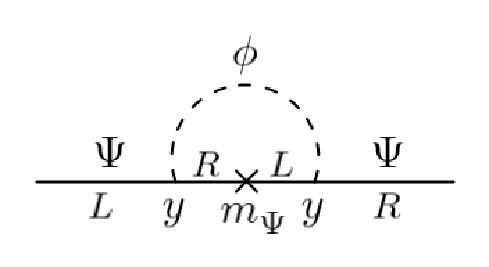
\includegraphics{Images/chiralityflip.pdf}
%     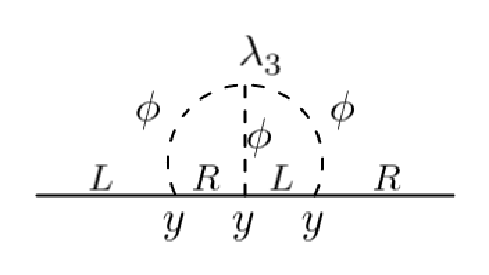
\includegraphics{Images/chiralityflip2.pdf}
%     %\caption{Diagrams for $\lambda_3=0$ and $\lambda_3\neq0$.}
%     }
% This interaction flips the chirality.\\
% $\bullet\lambda_3\neq0$:\;$\delta m_\Psi\prop\lambda_3y^3$, here we can use the \href{https://en.wikipedia.org/wiki/Hideki_Yukawa}{Yukawa} interaction to perform the chirality flip, we do not necessarily need the mass to do that.
% \end{exercise}
\section{The \href{https://en.wikipedia.org/wiki/Yoichiro_Nambu}{Nambu}-\href{https://en.wikipedia.org/wiki/Jeffrey_Goldstone}{Goldstone} Realization}
Another possible way to realize symmetries is the Nambu-Goldstone realization. We know that the equations of motion can have some symmetries but their solution will not necessarily be invariant under those symmetries. We talk about \textbf{Spontaneous Symmetry Breaking} (SSB) when the fundamental state is not symmetric while the Lagrangian is invariant under a certain symmetry. We look at the fundamental state because if it is not invariant, neither will be the excited states. SSB is usually associated with phase transitions.\\
To make things more clear, let's take a simple example in \textbf{Classical Mechanics}: consider a rod perpendicular to a flat surface. We apply a force to it and nothing initially happens, but if we increase the force the rod will bend in some random direction: the symmetric (unbent) configuration becomes unstable beyond this critical value of the force and the new ground state is asymmetric. Also, there are infinitely many possible degenerate ground states, related by rotational symmetry. We learnt that there is a critical value of the parameter beyond which we have SSB and that there is a manifold of degenerate vacua connected by symmetry transformations.\\
Let's move now to \textbf{Classical Field Theory}. The simplest relativistic system in which we can see SSB is one with a single scalar field with Lagrangian:
\[
\pazocal{L}=\frac{1}{2}(\partial_\mu\phi)^2-\underbrace{\left(\frac{\mu^2}{2}\phi^2+\frac{\lambda}{4}\phi^4\right)}_{V(\phi)}
\]
$\phi(x)$ is a real field, we want to find the configuration which minimizes the energy. Taking $\phi(x)=$ constant minimizes the kinetic energy, we have to look at the potential $V(\phi)$: for $\mu^2>0$, the system is invariant under parity $P_\phi:\phi\to-\phi$ and we have no SSB. What happens if $\mu^2<0$? $V(\phi)$ has some critical points:
\[
\frac{\partial V}{\partial\phi}=0=\mu^2\phi+\lambda\phi^3\Rightarrow
\left\{
\begin{aligned}
&\phi=0\\
&\phi=\pm\sqrt{-\mu^2/\lambda}=\pm v\xleftarrow[]{}\text{vacuum expectation value (vev)}
\end{aligned}
\right.
\]
$\phi=0$ corresponds to a maximum, while we have two minima in $\phi=\pm v$: the two fundamental states are \textbf{degenerate} and connected by a symmetry transformation $P_\phi: \phi=+v\to-\phi=-v$. The parameter in this case is $\mu^2$, the critical value is zero: for $\mu^2>0$ there is no SSB, for $\mu^2<0$ we have SSB.\\
How about SSB in \textbf{Quantum Mechanics}? Consider a particle in a double potential well $V(x)=\lambda(x^2-v^2)^2$. In this case we have tunnel effect connected to the amplitude of the maximum. Consider an Hamiltonian given by:
\[
H=\left(\begin{array}{cc}
    a & b \\
    b & a
\end{array}\right)
\]
such that $[P,H]=0$ in the subspace of the states $\ket{\pm v}$:
\[
\bra{v}H\ket{v}=a=\bra{v}P^2H\ket{v}=\bra{v}PHP\ket{v}=\bra{-v}H\ket{-v}
\]
If we have a particle confined in a well, there is a non-zero probability that after a certain time the particle will be in the other well. With similar arguments, we find:
\[
\bra{v}H\ket{-v}=\bra{-v}H\ket{v}=b
\]
After some mysterious calculations, $b$ turns out to be different from zero: this means that the eigenstates of $H$ must be combinations of $\ket{\pm v}$.
\[
\ket{\pm}=\frac{\ket{+v}\pm\ket{-v}}{2} \quad E_\pm=a\pm b
\]
Which one of these will be the fundamental state? using the nodes theorem, we see that for $b<0$ the fundamental state is $\ket{+}$ with $E_0=a+b$. Thanks to tunnel effect, we have only one fundamental state and it is no longer degenerate.\\
In \textbf{Quantum Field Theory} we can discretize the space\\
$\phi(x)\to\phi_m(x)=\phi(\Vec{x}_m,t)$, so that for each point we have a quantum mechanical variable. The tunnelling amplitude to get from $\+v$ to $-v$ will be proportional to $e^{-V}$ where $V$ is the volume of the space. Moving to continuum, the tunnelling probability goes to zero which means that if we are in a vacuum state of one of the two wells, we cannot go to the other one.\marginnote{There are some cases in QFT in which we have tunnelling but they are particular situations.} This allows us to have SSB, it is crucial to have an infinite number of variables in this situation.\\
Suppose to have a system with a large number of degrees of freedom. Realistically speaking, there will be some perturbation which gives us a small correction $\delta$ to the vacuum energy. $\delta$ is small compared to the experimental resolution but bigger than the off-diagonal terms which contribute to the tunnel effect. 
\subsection{Examples of SSB}
\labsec{exSSB}
\begin{example}
\textbf{Ferromagnet and the \href{https://en.wikipedia.org/wiki/Ernst_Ising}{Ising} model}\\
A ferromagnet can be described as a lattice of dipoles.\marginnote{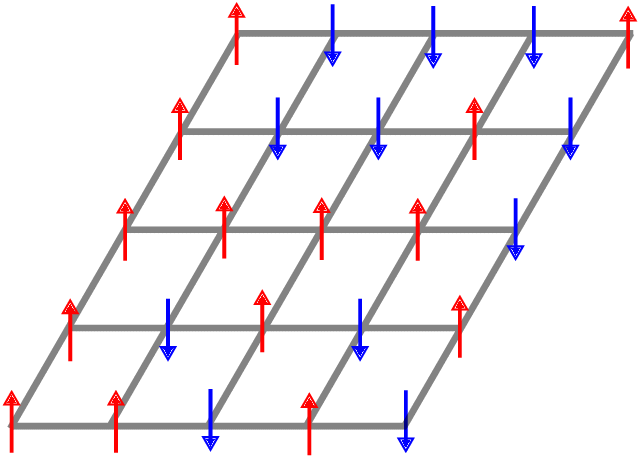
\includegraphics{Images/ising.png}}
\[
H=-\sum_{\{i,j\}}c_{ij}\Vec{\sigma}_i\cdot\Vec{\sigma}_j
\]
where the sum is extended over nearest neighbours and $c_{ij}$ are some positive valued coefficients. This is a scalar and therefore invariant under rotations. Such configuration depends on the temperature: for $T>T_c$, the dipoles are aligned randomly while for $T<T_c$ we have an ordered phase where all dipoles are aligned in the same direction. However, the ground state is one in which all the spins are aligned and all the degenerate ground states may by reached from a given one by a rotation. Suppose to start in a configuration where all the dipoles are aligned in a certain direction and we want to modify. We rotate some of them, by doing this we have a cost in energy: if we want to rotate all of them, we need to use an infinite amount of energy: there will be no tunnelling.
\end{example}
\begin{example}
\textbf{Linear U(1) sigma model}\marginnote{From \cite{schwartz}, Section 28.2.1.}\\
The simplest relativistic theory with SSB of a continuous global symmetry has a complex scalar field with Lagrangian:
\[
\pazocal{L}=\partial_\mu\phi^\dagger\partial^\mu\phi-\underbrace{\left(\mu^2\phi^\dagger\phi+\lambda(\phi^\dagger\phi)^2\right)}_{V(\phi)}
\]
This theory has a global U(1) symmetry given by $\phi\to e^{i\alpha}\phi$ with $\alpha\in[0,2\pi)$ and constant. For $\mu^2>0$, we have the minimum in the origin, a non interesting situation so we consider $\mu^2<0$. Define $\varphi^2:=\phi^\dagger\phi$ and look at the critical points of $V(\varphi)$:
\[
\frac{\partial V}{\partial\varphi}=2\mu^2\varphi+4\lambda\varphi^3=0\Rightarrow
\left\{
\begin{aligned}
&\varphi=0\\
&\varphi^2=-\frac{\mu^2}{2\lambda}\to\varphi=\frac{v}{\sqrt{2}}
\end{aligned}
\right.
\]
At the minimum, we have $\phi^\dagger\phi=\frac{v^2}{2}$. These vacuum states are all degenerate: $\phi(x)=\frac{1}{\sqrt{2}}ve^{i\theta}$, where $\theta$ is an arbitrary value describing the position of all the vacuum states in the manifold which are all connected by a symmetry transformation $\phi\to\phi+i\alpha\phi+\pazocal{O}(\alpha^2)$. The current associated is:
\[
J^\mu=\frac{\delta\pazocal{L}}{\delta(\partial_\mu\phi)}i\phi+\frac{\delta\pazocal{L}}{\delta(\partial\phi^\dagger)}(-i\phi^\dagger)=\partial_\mu\phi^\dagger i\phi-\partial_\mu\phi i\phi^\dagger=-i\phi^\dagger\overset{\leftrightarrow}{\partial_\mu}\phi
\]
All the vacua are equivalent (by symmetry) so it is possible to pick any convenient parametrization. Instead of writing $\phi(x)=v+\Tilde{\phi}(x)$, with $\Tilde{\phi}(x)$ a complex field, it is more convenient to expand around $v$ by parametrizing $\phi(x)$ in terms of two real fields $\eta(x)$ and $\xi(x)$:
\begin{equation}
\labeq{phipar}
\phi(x)=\frac{e^{i\xi(x)/v}}{\sqrt{2}}(v+\eta(x)) \quad \frac{\xi(x)}{v}\in[0,2\pi)
\end{equation}
$\phi(x)$ is a complex field, instead of writing $\pazocal{L}$ in terms of $\mathfrak{Re}\phi$ and $\mathfrak{Im}\phi$ we use a phase and an absolute value, with the latter given by $v+\eta(x)$ and $\langle\eta(x)\rangle=0$. We compute the Lagrangian in terms of the new variables:
\[
\left\{
\begin{aligned}
&\partial_\mu\phi=i\frac{\partial_\mu\xi(x)}{v\sqrt{2}}(v+\eta(x))e^{i\xi(x)/v}+\partial_\mu\eta(x)\frac{e^{i\xi(x)/v}}{\sqrt{2}}\\
&\partial_\mu\phi^\dagger\partial^\mu\phi=\frac{1}{2}(\partial_\mu\xi(x))^2\left(1+\frac{\eta(x)}{v}\right)^2+\frac{1}{2}(\partial_\mu\eta(x))^2\\
&V(\phi)=\frac{\mu^2}{2}(v+\eta(x))^2+\frac{\lambda}{4}(v+\eta(x))^4
\end{aligned}
\right.
\]
Putting all these pieces together we get:
\begin{align*}
\pazocal{L}=&\frac{1}{2}(\partial_\mu\xi(x))^2\left(1+\frac{\eta(x)}{v}\right)^2+\frac{1}{2}(\partial_\mu\eta(x))^2\\
&-\left[\lambda v^2\eta(x)^2+\lambda v\eta(x)^3+\frac{\lambda}{4}\eta(x)^4\right]\marginnote{We are not considering constant terms in the potential.}
\end{align*}
This Lagrangian describes a massless particle $\xi(x)$ as well as a massive particle $\eta(x)$. Some observations:
\begin{itemize}
    \item The field $\xi(x)$ has no potential but only the kinetic term, it represents the fluctuations around the valley of minima.
    \item The interactions of $\eta(x)$ are not invariant under $\eta(x)\to-\eta(x)$. Can we still talk about U(1) invariance? Not with this Lagrangian but we can define a transformation rule which implements the symmetry:
    \[
    \left\{
    \begin{aligned}
    &\xi(x)\to\xi(x)+v\alpha\\
    &\eta(x)\to\eta(x)
    \end{aligned}
    \right.
    \]
    This is still a U(1) transformation, non homogeneous and in general non linear. The fields are not invariant but at the Lagrangian level symmetry is still present, we just realized it in an unusual way. At quantum level, $\xi(x)$ describes massless scalars called \textbf{Nambu-Goldstone bosons} (NGB). The field $\eta(x)$ can be visualized as radial excitations of the potential shown on the side, commonly called a Mexican hat potential.\marginnote[-2cm]{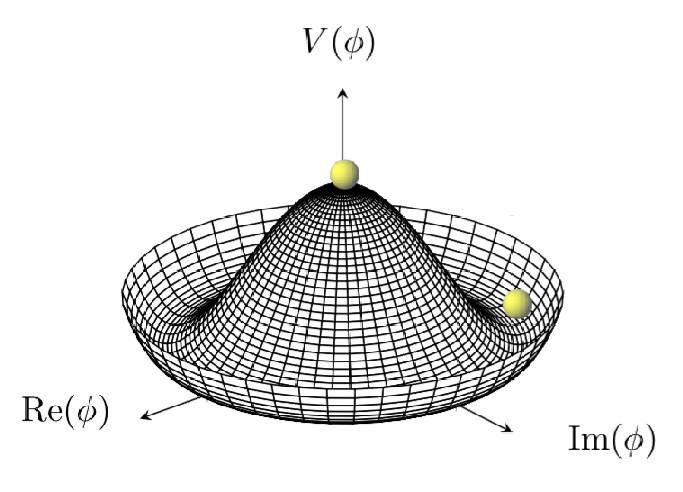
\includegraphics[]{Images/sombrero.png}}
    \item The manifold where $\xi(x)$ lives is the manifold of vacua ($\sim$S$^1$)
\end{itemize}
Massless Goldstone bosons such as $\xi(x)$ will appear in any theory with SSB (by Goldstone theorem [\refthm{GT}]), with one massless particle for each broken symmetry. Goldstone bosons are naturally associated with shift symmetries: it is easy to see from \refeq{phipar} that a phase rotation in $\phi(x)$ amounts to a shift in $\xi(x)$. The shift symmetry forbids a mass term for $\xi(x)$. There is a close connection between Goldstone theorem and shift symmetries of the Goldstone bosons. We now want to write the current in terms of $\xi(x)$ and $\eta(x)$:
\[
\left\{
\begin{aligned}
&\partial_\mu\phi=i\frac{\partial_\mu\xi(x)}{v\sqrt{2}}(v+\eta(x))e^{i\xi(x)/v}+\partial_\mu\eta(x)\frac{e^{i\xi(x)/v}}{\sqrt{2}}\\
&\phi^\dagger\partial_\mu\phi=i\frac{\partial_\mu\xi(x)}{2v}(v+\eta(x))^2+\frac{1}{2}(\partial_\mu\eta(x))(v+\eta(x))
\end{aligned}
\right.
\]
Putting everything together gives us:
\[
J^\mu=-\cancel{2}i\frac{i\partial_\mu\xi(x)}{\cancel{2}v}(v+\eta(x))^2=v\partial_\mu\xi(x)+(\text{higher orders in the fields})
\]
The current is interpolating the NGB, the U(1) symmetry has been broken into the identity.
\end{example}
\begin{example}
\textbf{Linear O(N) sigma model}\marginnote{Facciamo finta che questo esempio abbia senso ed andiamo avanti.}\\
Consider a theory of $N$ real scalar fields:
\[
\pazocal{L}=\frac{1}{2}(\partial_\mu\phi_i)(\partial^\mu\phi_i)-\underbrace{\left(\frac{\mu^2}{2}\phi_i\phi_i+\frac{\lambda}{4}(\phi_i\phi_i)^2\right)}_{V(\phi)}
\]
with $\mu^2<0$. In this case, we have a SO$(N)$ symmetry: $\phi\to e^{iT^a\alpha^a}\phi$, $T^a\in\mathfrak{so}(N)$. The vacuum is described by $\phi(x)=\phi_0=\begin{pmatrix}0\\0\\ \vdots\\v\end{pmatrix}$ which corresponds to choosing a particular direction in the valley of minima and we can always do this since we have invariance under rotations. Conventionally, we choose coordinates so that we have $\phi_0$ in the n-th direction. Its absolute value is given by $\phi_0^T\phi_0=v^2=-\mu^2/\lambda$ and it is invariant under SO$(N-1)$. Look now at the current $J^{\mu,A}$ and the charge associated $Q^A=\int d^3xJ^{0,A}(\Vec{x},t)$: does $e^{iQ^A\alpha}$ leave the vacuum invariant? The ones leaving it invariant are transformations of SO(N-1).
\begin{align*}
&\bullet \text{SO}(N-1):\; \frac{(N-1)(N-1-1)}{2} \quad \text{\# (unbroken) generators}\\
&\bullet \text{SO}(N):\;\frac{N(N-1)}{2} \quad \text{\# generators}\\
&\bullet \frac{N(N-1)}{2}-\frac{(N-1)(N-2)}{2}=N-1 \quad \text{\# broken generators}
\end{align*}
This $N-1$ broken generators are the ones which do not leave the vacuum invariant. We can write $\phi(x)$ as:
\[
\phi(x)=e^{i\xi^{\hat{a}}(x)T^{\hat{a}}/v}\begin{pmatrix}0\\0\\ \vdots\\v+\eta(x)\end{pmatrix}
\]
We want in total $N$ fields, these are given by the $N-1$ fields $\xi^{\hat{a}}(x)$+the absolute value of $\phi(x)$. The fields $\xi^{\hat{a}}(x)$ do not have a potential while $\eta(x)$ are massive and they will have interactions which do not involve derivatives. We can remove the generators that leave the vacuum invariant:
\[
iT^a=\left(
\begin{array}{cccc}
& & & 0\\
& \bigita & & \vdots\\
& & & \vdots\\
0&\dots&\dots &0\\
\end{array}
\right)
\quad
iT^{\hat{a}}=\left(
\begin{array}{ccccc}
& & & & 0\\
& &\bigzero & & \vdots\\
& & & & 1\\
& & & & \vdots\\
0&\dots& -1 &\dots &0\\
\end{array}
\right)
\]
$T^a,t^a\in\mathfrak{so}(N-1)$, we have the generators only on the $(N-1)\times(N-1)$ block above. $T^{\hat{a}}\in\mathfrak{so}(N)$ but $T^{\hat{a}}\not\in\mathfrak{so}(N-1)$, the 1 and -1 are present in the matrix above only on row $\hat{a}$ and column $\hat{a}$. SO(N) is broken into SO(N-1). It is useful to expand $\phi(x)$ at the first order in the fields:
\[
\phi(x)\simeq\left(\begin{array}{c}
     \xi^1(x)\\
     \xi^2(x)\\
     \vdots\\
     \xi^{n-1}(x)\\
     v+\eta(x)
\end{array}\right)+\text{higher orders in the fields}
\]
$\xi^{\hat{a}}(x)$ are massless and have no potential, they are excitations in the valley of minima, i.e. Goldstone bosons. We saw for the U(1) case that the current can interpolate them, we want to see it for SO(N) too.
\[
J^{\mu,A}=\frac{\delta\pazocal{L}}{\delta(\partial_\mu\phi_i)}iT_{ij}^A\phi_j=\partial_\mu\phi_iiT_{ij}^A\phi_j
\]
We want to compute the current for the broken generators.
\[
\partial_\mu\phi_i=i\frac{\partial_\mu\xi^{\hat{a}}(x)}{v}T^{\hat{a}}_{ik}\phi_k+(e^{i\xi^{\hat{a}(x)}T^{\hat{a}}/v}\phi_0)_i\frac{\partial_\mu\eta(x)}{v}
\]
When plugging this in the expression for the current, the second term disappears due to the anti-symmetry of $T_{ij}^{\hat{a}}$ so we are left with:
\[
J^{\mu,\hat{a}}=i\frac{\partial_\mu\xi^{\hat{b}}(x)}{v}T_{ik}^{\hat{b}}\phi_kiT_{ij}^{\hat{a}}\phi_j\underset{\mathclap{\tikz \node {$\uparrow$} node [below=1ex] {\footnotesize  swap $k$ and $i$, giving a - sign};}}{=}\frac{\partial_\mu\xi^{\hat{b}}(x)}{v}\overbrace{\phi_kT_{ki}^{\hat{b}}T_{ij}^{\hat{a}}\phi_j}^{\phi^TT^{\hat{b}}T^{\hat{a}}\phi}
\]
We now expand the term highlited in fancy curly brackets:
\begin{align*}
\phi^TT^{\hat{b}}T^{\hat{a}}\phi&\simeq\phi_0^TT^{\hat{b}}T^{\hat{a}}\phi_0=\phi_0^T\frac{(T^{\hat{b}}T^{\hat{a}}+T^{\hat{a}}T^{\hat{b}})}{2}\phi_0=\frac{1}{2}\phi_0^T\{T^{\hat{a}},T^{\hat{b}}\}\phi_0\\
&=\frac{1}{2}\phi_0^T2\delta_{ab}\phi_0=\phi_0^T\phi_0\delta_{ab}=v^2\delta_{ab}
\end{align*}
Which at the end of the day gives us:
\[
J^{\mu,\hat{a}}=v\partial_\mu\xi^{\hat{a}}(x)+\text{higher orders}
\]
which is exactly what we wanted to show, the broken currents interpolates the NGBs. The number of NGBs is equal to the number of broken currents, in this case (N-1). This is a general rule. As in the U(1) case, the manifold of vacua is the same as the manifold of NGBs: what is the manifold of vacua here? We have SO(N) rotations, by moving a unitary vector we have $S^{N-1}$ and the NGBs are fluctuations in this sphere with no energy cost. NGBs transform non linearly under SO(N), let's look at the transformation rules.\marginnote{A is for broken generators, V is for the unbroken generators.}
\[
\phi(x)=e^{i\xi(x)\cdot A}\left(1+\frac{\eta(x)}{v}\right)\phi_0\xrightarrow[g\in\text{SO}(N)]{}g\phi(x)=ge^{i\xi(x)\cdot A}\left(1+\frac{\eta(x)}{v}\right)
\]
We want to understand how to write the transformed NGB: any $g\in$G can be written as $T_1=e^{i\alpha\cdot A}e^{i\beta\cdot V}$ where $A\in\mathfrak{g}$ and $V\in\mathfrak{h}$, with H$\le$G.
\[
ge^{i\xi(x)\cdot A}=e^{i\xi'(\xi,g)\cdot A}e^{iu(\xi,g)\cdot V}
\]
We denoted with $\xi'(\xi,g)$ the transformed NGB.
\[
\phi'(x)=g\phi(x)=e^{i\xi'(\xi,g)\cdot A}\underbrace{e^{iu(\xi,g)\cdot V}}_{\in\text{H=SO}(N-1)}\phi_0\left(1+\frac{\eta(x)}{v}\right)
\]
The term in SO$(N-1)$ leaves the vacuum invariant by definition, hence we have:
\[
\phi'(x)=e^{i\xi'(\xi,g)\cdot A}\phi_0\left(1+\frac{\eta(x)}{v}\right)
\]
The NGB does not transform linearly, so we found two ways of realizing a symmetry: linearly (Weyl) and non-linearly (depends on the NGB).
\end{example}
\section{SSB in QFT}
At this point we want to quantize the theory and introduce the \textbf{Goldstone theorem}, valid also in QCD. We have already seen how to quantize the theory in the case of linearly realized symmetries: using the N\"other's theorem, we are able to compute the charge starting from the current. In the Wigner-Weyl realization we know that the current is conserved and the charge is well defined and conserved. We now want to see the case in which the charge does \textbf{not annihilate} the vacuum anymore, so that we cannot use Coleman's theorem [\refthm{Coleman}] and the charge will no longer be conserved. We make some assumptions:
\begin{enumerate}
    \item $S_{\text{classical}}$ is invariant under a certain symmetry
    \item $\partial_\mu J^{\mu,a}(x)=0$ as operator
    \item $Q^a\ket{0}\neq0$ for some charges.
\end{enumerate}
Suppose now to have two charges, $Q^a$ and $Q^b$, which both annihilate the vacuum:
\[
[Q^a,Q^b]\ket{0}=0 \quad [Q^a,Q^b]=if^{abc}Q^c
\]
The charges which annihilate the vacuum generate a linearly realized symmetry subgroup called H. The other charges do not annihilate the vacuum, they are not well defined [\refthm{FP}] and the integral is not convergent, but it is possible to define a regularized version of the integral:
\[
Q^a=\int d^3xJ^{0,a}(\Vec{x},t)\xrightarrow[\text{regularization}]{}Q^a_V(t)=\int_V d^3xJ^{0,a}(\Vec{x},t)
\]
The regularized version of the charge will no longer be conserved because it depends on the time. What we can do instead is to look at the commutator of the charge with a local operator $A$ located in a point $A(y)$ or in a finite space-time region.
\[
[Q_V^a(t),A(y)]=\lim_{V\to\infty}\int_Vd^3x[J^{0,a}(\Vec{x},t),A(y)]\stackrel{?}{<}\infty
\]
We ask ourselves whether this integral is convergent or not. For relativistic QFT, microcausality tells us that $[O_1(x),O_2(y)]=0$ for $(x-y)^2<0$, i.e. $x,y$ space-like. As $V\to\infty$, we will get $(x-y)^2<0$ so the integral will converge and the commutator of the charge with any local operator is well defined. If we fix a time such that $x$ and $y$ are space-like we must be out of the light cone, but this will eventually happen as we are integrating over $V\to\infty$. We can extend this reasoning to a local operator located in a finite space-time region by considering all the light cones centered in the points of such region and there will always be a $x$ large enough to make the integrand zero in every point of the region.\\
Moreover, we can also prove prove that this commutator does not depend on time.
\begin{align*}
\frac{d}{dt}[Q_V^a(t),A]&=\lim_{V\to\infty}\int_Vd^3x\left[\frac{\partial}{\partial t}J^{0,a}(\Vec{x},t),A(y)\right]\\
&\underset{\mathclap{\tikz \node {$\uparrow$} node [below=1ex] {\footnotesize $\partial_\mu J^\mu=0$ };}}{=}\lim_{V\to\infty}\int_Vd^3x[\Vec{\nabla}\cdot\Vec{J}(\Vec{x},t),A(y)]\\
&=\lim_{V\to\infty}\int_{\partial V}dS[\hat{n}\cdot\Vec{J}(\Vec{x},t),A(y)]=0
\end{align*}
Due to microcausality, $(x-y)^2<0\;\forall x\in\partial V$.
% Consider now the operator $A$ to have some transformation rules under a certain symmetry:
% \[
% A\to U(\alpha)AU^{-1}(\alpha) \quad U(\alpha)=\exp{iQ^a\alpha^a}
% \]
% In our case, $Q^a$ is not well defined, we can apply this rule only in the Wigner-Weyl realization. Nevertheless we can work with the regularized version of the charge and see what happens to this transformation when sending $V\to\infty$.
% \begin{align*}
% \lim_{V\to\infty}U_V(\alpha)AU^{-1}_V(\alpha)&=\lim_{V\to\infty}e^{iQ_V^a\alpha^a}Ae^{-iQ_V^a\alpha^a}\\
% &\simeq\lim_{V\to\infty}\left[A+i\alpha^a[Q_V^a,A]+\frac{i^2}{2}\alpha^a\alpha^b[Q_V^b,[Q_V^a,A]]+\dots\right]
% \end{align*}
% By defining $\delta_aA:=\lim_{V\to\infty}[Q_V^a,A]$, we can write the transformation as $A\to A+i\alpha^a\delta_aA$. The vacuum expectation value of the transformed $A$:
% \[
% \lim_{V\to\infty}\bra{0}U_V(\alpha)AU_V^{-1}(\alpha)\ket{0}=\lim_{V\to\infty}\bra{\alpha_V}A\ket{\alpha_V}
% \]
% can be seen as the limit for the transformed state $\ket{\alpha_V}$ given by\\ $\ket{\alpha_V}:=U_V^{-1}(\alpha)\ket{0}$. However, the limit of this quantity does not exist but we can overcome this problem by considering both states and taking the limit, but we cannot take the limit singularly of $\ket{\alpha_V}$. We can still consider the vacuum expectation value of some observable $A$ and the vacuum expectation value of the transformed observable $Ag^{-1}$, which can be interpreted as the vacuum expectation value on the transformed state after taking the limit of $V\to\infty$. This is the expectation value of the transformed state, but we cannot directly transform it. This is because the Hilbert space must be \textbf{separable}, i.e. it must contain a countable number of basis vectors. Each vacuum state can be used to create a Hilbert space, different vacuum states contribute to different theories hence a rotation would bring our state in a space which is not the one of our theory. $Q^a\ket{0}$ is not a state on our Hilbert space, but we can still work with the expectation value of the transformed operator.
All this machinery is needed to prove the Goldstone Theorem.
\subsection{Goldstone Theorem}
\label{GT}
\begin{theorem}
\labthm{GT}
Spontaneous breaking of continuous global symmetries implies the existence of massless particles. Equivalently, for any regularized charge $Q_V^a$ such that $\lim_{V\to\infty}Q_V^a\ket{0}\neq0$ there exists a massless particle, the Nambu-Goldstone Boson (NGB). 
\end{theorem}
\marginnote{From \cite{R}, Section 8.2.}If the Lagrangian is invariant under a group transformation, then the currents have zero divergence $\partial_\mu J^{\mu,a}=0$, the corresponding charges are conserved and they have the commutation relations of symmetry group. If the vacuum is invariant under the group, i.e. a singlet, the charges annihilate the vacuum. This is the usual case for a symmetry. If this is not the case, we say that we have degenerate vacua.
\begin{proof}
\marginnote{\href{https://physics.stackexchange.com/questions/417753/schwartzs-and-zees-proof-of-goldstone-theorem}{This post} from Physics StackExchange can be useful.}The Goldstone theorem states that if there exists such a charge, then there is a field operator $\phi'(x)$ with non-vanishing vacuum expectation value $\bra{0}\phi'(x)\ket{0}\neq0$ and which is not a singlet under the transformation of some symmetry group.  Since $\phi'(x)$ is not a singlet under the group, there must exist an operator $\phi(x)$ such that:
\[
[Q_V^a,\phi(x)]=\phi'(x)
\]
$\phi'(x)$ have a non-vanishing vacuum expectation value, from which it follows that:
\[
\bra{0}[Q_V^a,\phi(x)]\ket{0}\neq0
\]
We now show that this condition implies the existence of massless particles. Our starting point is the explicit computation of the vacuum expectation value of this commutator. We use the definition of charge and insert a complete set of intermediate states:
\[
\lim_{V\to\infty}\sum_n\int_V d^3y\left[\bra{0}J^{0,a}(y)\ket{n}\bra{n}\phi(x)\ket{0}-\bra{0}\phi(x)\ket{n}\bra{n}J^{0,a}(y)\ket{0}\right]\neq0
\]
Translation invariance implies that $J^\mu(y)=e^{-ipy}J^\mu(0)e^{+ipy}$ so that the previous expression becomes:
\begin{align*}
&\lim_{V\to\infty}\sum_n\int_V d^3y\left[\underbrace{\bra{0}e^{-ipy}}J^{0,a}(0)\underbrace{e^{+ipy}\ket{n}}\bra{n}\phi(x)\ket{0}-\bra{0}\phi(x)\ket{n}\underbrace{\bra{n}e^{-ipy}}J^{0,a}(0)\underbrace{e^{+ipy}\ket{0}}\right]\\
=&\lim_{V\to\infty}\sum_n\int_V d^3y\left[\bra{0}J^{0,a}(0)\ket{n}\bra{n}\phi(x)\ket{0}e^{+ip_ny}-\bra{0}\phi(x)\ket{n}\bra{n}J^{0,a}(0)\ket{0}e^{-ip_ny}\right]\neq0
\end{align*}
We used the assumption that the vacuum has zero energy when applying $e^{\pm ipy}$. It is now possible to perform the spatial integration, which gives us:
\begin{align*}
&\sum_n(2\pi)^3\delta^3(\Vec{p}_n)\left[\bra{0}J^{0,a}(0)\ket{n}\bra{n}\phi(x)\ket{0}e^{iE_ny^0}-\bra{0}\phi(x)\ket{n}\bra{n}J^{0,a}(0)\ket{0}e^{-iE_ny^0}\right]\neq0
\end{align*}
Previously, we used microcausality to show that the commutator of the charge with a local operator is independent on time. Now we require the same condition, so we compute the derivative with respect to $y^0$ and impose that it is equal to zero.
\begin{align*}
\frac{\partial}{\partial y^0}\bra{0}[Q_V^a,\phi(x)]\ket{0}&=\frac{\partial}{\partial y^0}\sum_n(2\pi)^3\delta^3(\Vec{p}_n)\left[\bra{0}J^{0,a}(0)\ket{n}\bra{n}\phi(x)\ket{0}e^{iE_ny^0}-\bra{0}\phi(x)\ket{n}\bra{n}J^{0,a}(0)\ket{0}e^{-iE_ny^0}\right]\\
&=\sum_ni(2\pi)^3\delta^3(\Vec{p}_n)E_n\left[\bra{0}J^{0,a}(0)\ket{n}\bra{n}\phi(x)\ket{0}e^{iE_ny^0}+\bra{0}\phi(x)\ket{n}\bra{n}J^{0,a}(0)\ket{0}e^{-iE_ny^0}\right]
\end{align*}
The two conditions $\bra{0}[Q_V^a,\phi(x)]\ket{0}\neq0$ and $\frac{\partial}{\partial y^0}\bra{0}[Q_V^a,\phi(x)]\ket{0}=0$ are compatible if:
\[
\left\{
\begin{aligned}
&\bra{0}J^{0,a}(0)\ket{n}\bra{n}\phi(x)\ket{0}=0\quad &&\text{for}\;E_n\neq0\\
&\bra{0}J^{0,a}(0)\ket{n}\bra{n}\phi(x)\ket{0}\neq0\quad &&\text{for}\;E_n=0
\end{aligned}
\right.
\]
The last constraint is telling us that $\ket{n}$ is a massless 1-particle state. Why? Because what must be equal to zero is the product:
\[
\delta^3(\Vec{p}_n)E_n\underset{\mathclap{\tikz \node {$\uparrow$} node [below=1ex] {\footnotesize for $N$ particles };}}{=}\delta^3\left(\sum_{k=1}^N\Vec{p}_k\right)\left(\sum_{k=1}^N\sqrt{m_k^2+|\Vec{p}_k|^2}\right)
\]
The only way in which this can be zero is to have only \textbf{one massless particle}, $\delta^3(\Vec{p}_n)\sqrt{m_n^2+|\Vec{p}_n|^2}=0$ when $m_n=0$. The two conditions we required are satisfied only by massless one-particle states. Multi-particle states does not give us $\frac{\partial}{\partial y^0}\bra{0}[Q_V^a,\phi(x)]\ket{0}=0$ because the total momentum will be the sum of the momentum of each particle which is different from zero, implying energy different from zero even if they are massless.\\   
Let's keep only the contribution coming from massless one-particle states $\chi^b(\Vec{p})$ and see if we can obtain some more information. For one-particle states we have:
\[
\sum_n\to\int\frac{d^3p}{(2\pi)^3}\frac{1}{2E_p}
\]
where $E_p$ is the energy of the single particle. This means that:
\begin{align*}
\bra{0}[Q_V^a,\phi(x)]\ket{0}=\int\frac{d^3p}{\cancel{(2\pi)^3}}\frac{\cancel{(2\pi)^3}}{2E_p}\delta^3(\Vec{p})&\left[\bra{0}J^{0,a}(0)\ket{\chi^b(\Vec{p})}\bra{\chi^b(\Vec{p})}\phi(x)\ket{0}e^{iE_pt}\right.\\
&\left.-\bra{0}\phi(x)\ket{\chi^b(\Vec{p})}\bra{\chi^b(\Vec{p})}J^{0,a}(0)\ket{0}e^{-iE_pt}\right]
\end{align*}
We want to write the matrix elements using Lorentz invariance:
\begin{equation}
\labeq{leftpart}
\bra{0}J^{\mu,a}(x)\ket{\chi^b(\Vec{p})}=iF_{ab}p^\mu e^{ipx} \quad \bra{\chi^b(\Vec{p})}\phi(x)\ket{0}=Z_{ab}
\end{equation}
For the first matrix element, keep in mind that $\partial_\mu J^\mu=0$ so when deriving there is another factor $p^\mu$. There will be $p^2$ but since we are dealing with massless particles, the derivative of this matrix element will be equal to zero. Now we plug this in $\bra{0}[Q_V^a,\phi(x)]\ket{0}$, remembering that for massless particles $p^\mu=p^0=E_p$:
\[
\bra{0}[Q_V^a,\phi(x)]\ket{0}=\int\frac{d^3p}{2\cancel{E_p}}\delta^3(\Vec{p})\left[iF_{ab}\cancel{E_p}Z_{ab}e^{iE_pt}+iZ_{ab}F_{ab}\cancel{E_p}e^{-iE_pt}\right]
\]
We evaluate the integral:
\[
\int d^3p\delta^3(\Vec{p})e^{iE_pt}=1
\]
Similarly, for $\frac{\partial}{\partial y^0}\bra{0}[Q_V^a,\phi(x)]\ket{0}$ we obtain the integral:
\[
\int d^3p\delta^3(\Vec{p})E_pe^{iE_pt}=0
\]
So, in the limit $V\to\infty$, we get
$\bra{0}[Q_V^a,\phi(x)]\ket{0}=iF_{ab}Z_{ab}$ while its derivative with respect to $y^0$ is equal to zero.\\
In general, there will be an unbroken subgroup H$\subset$G which linearly realizes the symmetry, where G is the symmetry group: both $J^{\mu,a}$ and $\chi^b$ transform as some representation of the unbroken group. But the left part of \refeq{leftpart} tells us that $J^{\mu,a}$ is interpolating $\chi^b$ from the vacuum and since they both transform as a representation of the unbroken group, this representation must be the same, being the vacuum Lorentz invariant.\\
Charges are the generators of the symmetry group, if they do not annihilate the vacuum it means that the vacuum is not invariant under the action of the symmetry group and we have SSB. The charges which annihilate the vacuum form a linearly realized symmetry subgroup, while the other charges \textit{breaks} the initial symmetry, with one current associated to each charge which correspond to a massless one-particle state.
\begin{kaobox}[frametitle=\#NGB]
\[
\text{\#NGB = \#broken currents = \#broken generators}
\]
\end{kaobox}
\end{proof}
% Denote now with $U(\beta)$ the unitary operator which implement the transformation in the linearly realized symmetry subgroup H.
% \[
% \bra{0}J^{\mu,a}(x)\ket{\chi^b(\Vec{p})}=\bra{0}\underbrace{U(\beta)J^{\mu,a}(x)U^{-1}(\beta)}_{{\color{red}{\text{transformed current}}}}\overbrace{U(\beta)\ket{\chi^b(\Vec{p})}}^{{\color{blue}{\text{transformed state}}}}={\color{red}{R_{aa'}}}{\color{blue}{R_{bb'}}}\bra{0}J^{\mu,a'}(x)\ket{\chi^{b'}(\Vec{p})}
% \]
% In the first step we used the fact that the vacuum is invariant under this transformation, $R_{aa'}$ is a matrix representing the current transformation, $R_{bb'}$ is a matrix for the state transformation. These two matrices must be the same since the state and the current must undergo the same transformation. This means that $F_{ab}=R_{aa'}R_{bb'}F_{a'b'}$, $F_{ab}$ is an invariant tensor under transformations of H.\\
% \begin{example}
% In SO$(N)$ the transformation $R$ is a rotation of SO$(N-1)$. Let SO$(N-1)$=H: $F_{ab}=F\delta_{ab}$, where $F$ is the decay constant of the NGB. There is only one parameter for all the NGBs, this is because of the covariance under SO$(N-1)$ so we do not need an elaborate matrix but just a number. We repeat the same argument for the other matrix element:
% \[
% \bra{\chi^b(\Vec{p})}\phi_i(x)\ket{0}=Z_{ib}
% \]
% In this example, we can choose as SO$(N-1)$ the rotations of the first $N-1$ indices: $i=1,\dots,N$ ($N$ fields) and $b=1,\dots,N-1$ ($N-1$ NGBs). Setting $i=N$ means having $Z_{Nb}=0$ because we have no vector for $N$, while $Z_{ab}=Z\delta_{ab}$ for $i=a$. We have only two quantities, $F$ and $Z$ and it is always possible to renormalize $\phi_i$ to have $Z=1$. If we now compute the order parameter we get $\langle T_{ij}^a\phi_j\rangle=iF\delta_{ia}$ where $T_{ij}^a=i(\delta_{ai}\delta_{jN}-\delta_{aj}\delta_{iN})$ are the broken generators. From this, we get $\langle\phi_j\rangle=F\delta_{jN}$ which is different from zero only for the last component, as we assumed, according with the fact that a SO$(N-1)$ rotation involves only the first $N-1$ components.
% \end{example}
We proved the existence of this massless particle which must have the same quantum numbers of the current $J^{\mu,a}(x)$ and the scalar field $\phi(x)$. It is possible to excite the particle using both operators, which are two apparently different things but actually they are not because we have to look at transformation rules under the unbroken subgroup which linearly realizes the symmetry.\\
SO$(N-1)$. $J^{\mu,a}$ transforms as the fundamental of SO$(N)$, $\phi_i(x)$ is in the fundamental of SO$(N)$ which gets broken in the fundamental of SO$(N-1)$+a singlet. Two different operators can excite the same particle, the fact that $\phi_i(x)$ is a scalar field (otherwise it would break Lorentz invariance for the vacuum) is telling us that this particle must be a boson. \marginnote{In supersymmetry theory, the field is fermionic.}
Goldstone theorem does not imply that these particles must be in the physical spectrum, it just states that they must exist.\\
An alternative proof of the Goldstone theorem is the following.\marginnote{This alternative proof is terrible, stick to the previous one.}
\begin{proof}
Start by computing:
\begin{align*}
\partial_\mu^x\bra{0}T[J^{\mu,a}(x)\phi_i(0)]\ket{0}&=\partial_\mu^x\left[\theta(x^0)\bra{0}J^{\mu,a}(x)\phi_i(0)\ket{0}+\theta(-x^0)\bra{0}\phi_i(0)J^{\mu,a}(x)\ket{0}\right]\\
&=\delta(x^0)\bra{0}[J^{0,a}(x),\phi_i(0)]\ket{0}
\end{align*}
Now we integrate:
\[
\int d^4x\partial_\mu^x\bra{0}T[J^{\mu,a}(x)\phi_i(0)]\ket{0}=\bra{0}[Q^a,\phi_i(0)]\ket{0}=\langle\delta_a\phi_i\rangle\neq0
\]
This is different from zero because of the presence of the massless state. We write the matrix element in \href{https://en.wikipedia.org/wiki/Joseph_Fourier}{Fourier} space.
\[
\bra{0}T[J^{\mu,a}(x)\phi_i(0)]\ket{0}=\int\frac{d^4p}{(2\pi)^4}e^{ipx}G^{\mu,a,i}(p)\xleftarrow[]{}\text{FT of the T-product, i.e. Green's function}
\]
Using Lorentz covariance, we write $G^{\mu,a,i}(p)=-ip^\mu H^{a,i}(p^2)$ and substitute it in the first integral.
\[
\int d^4pp^2\delta^4(p)H^{a,i}(p^2)
\]
If $H^{a.i}(p^2)$ has no poles the integral goes to zero, so it must be:
\[
H^{a,i}(p^2)=\frac{\langle\delta_a\phi_i\rangle}{p^2}+\text{regular terms in $p^2$}
\]
We are exciting the field in a point with the current and with $\phi_i$ in another point. The existence of the pole implies the existence of a state interpolated from the vacuum by $J^\mu$ and $\phi_i$, which propagates and gives us the pole: this is the NGB.\\
\end{proof}
\textbf{Remarks:}
\begin{enumerate}
    \item We cannot have SSB of a symmetry (discrete or continue) in dimension $d\le2$ because of infrared divergence.
    \item How do we know if we have SSB in our theory? At the classical level, we check the derivative of the potential and look for the minima. In general, we have to look at the effective potential which includes radiative corrections, and look for the minima.
\end{enumerate}
\end{document}



%QFT beyond tree-level (QED a 1 -loop con Barducci)
%Symmetries and conservation laws (spontaneous symmetry breaking and Higgs mechanism)
%Quick intro to non-abelian gauge theories
%Effective field theories
%Intro to the SM